\documentclass{exam}
 
\usepackage{graphicx}
\usepackage{float}
\usepackage{amsmath}
\usepackage{subcaption}
\usepackage{framed}
\usepackage{algorithm2e}
\usepackage{algpseudocode}
 
% First we setup the header and footer
\pagestyle{headandfoot}
\runningheadrule
\runningfootrule
\header{CSE101: Design and Analysis of Algorithms (CSE, UCSD, Summer-2020)}{}{Homework-03}
\footer{}{\thepage  \, of \numpages}{}
 
% We want the points for each question displayed on the left
%\pointname{points}
%\pointsinmargin
 
% Automatically total the points - make sure to compile TWICE
\addpoints
 
\begin{document}


\begin{center} 
\fbox{\parbox{5.5in}{
\vspace{-0.1in}
\begin{itemize}
\item \small{The instructions are the same as in Homework-0, 1, 2.}
\end{itemize}
\vspace{-0.1in}
}}
\end{center}

\vspace{0.1in}


\vspace{0.1in}
% Some general text together with number of questions and total points possible
There are \numquestions\, questions for a total of \numpoints\, points.
\vspace{0.1in}
\hrule
 \vspace{0.2in}
\begin{questions}
 
% First question, worth 3 points
\question Counterexamples  are effective in ruling out certain algorithmic ideas. In this problem, we will see a few such cases.

\begin{parts}
\part[5] Recall the following event scheduling problem discussed in class (lecture 15): 
\begin{quote}
You have a conference to plan with $n$ events and you have an unlimited supply of rooms. Design an algorithm to assign events to rooms in such a way as to minimize the number of rooms.
\end{quote}
The following algorithm was suggested during class discussion.
\begin{framed}
{\tt ReduceToSingleRoom($E_1, ..., E_n$)}\\
\hspace*{0.1in} - $U \leftarrow \{E_1, ..., E_n\}$; $i \leftarrow 1$\\
\hspace*{0.1in} - While $U$ is not empty:\\
\hspace*{0.3in} - Use Earliest Finish Time greedy algorithm on events in set $U$ \\
\hspace*{0.4in} to schedule a subset $T \subseteq U$ of events in room $i$\\
\hspace*{0.3in} - $i \leftarrow i + 1$; $U \leftarrow U \setminus T$
\end{framed}
Show that the above algorithm does not always return an optimal solution.\\

Consider the case when we have event's timeslots as 1-2, 1-3, 2-5, and 3-4. The algorithm will first choose 1-2 based on the earliest finish time and then choose an event that doesn't have any time conflict which is 3-4. On the next pass, the algorithm will choose 1-3 for the same reason. Lastly, it will choose 2-5. The algorithm has scheduled the events into 3 rooms. However, based on observation, we can arrange events 1-2 and 2-5 into room 1, events 1-3 and 3-4 into room 2 so only 2 rooms are needed in total, which is a counterexample. Thus the algorithm does not always return an optimal solution.

\vspace{0.5in}


\part[5] A longest simple path from a node $s$ to $t$ in a weighted, directed graph is a simple path from $s$ to $t$ such that the sum of weights of edges in the path is maximised. Here is an idea for finding a longest path from a given node $s$ to $t$ in any weighted, directed graph $G=(V, E)$:
\begin{quote}
Let the weight of the edge $e \in E$ be denoted by $w(e)$ and let $w_{max}$ be the weight of the maximum weight edge in $G$. Let $G'$ be a graph that has the same vertices and edges as $G$ but for every edge $e \in E$, the weight of the edge is $(w_{max} + 1 - w(e))$. ({\it For example, consider the graph $G$ below and its corresponding graph $G'$.})
\begin{center}
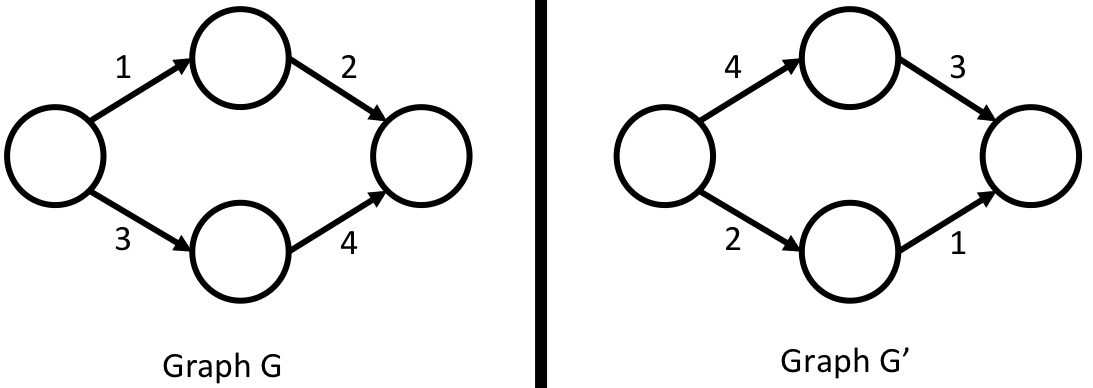
\includegraphics[scale=0.25]{dijk}
\end{center}
Run Dijkstra's algorithm on $G'$ with starting vertex $s$ and return the shortest path from $s$ to $t$.
\end{quote}

Show that the above algorithm does not necessarily  output the longest simple path.\\

Consider the case when we add a directed edge of weight 3 from the top-most node to the bottom-most node in $G$. Then, according to the algorithm, we will add a directed edge of weight 2 from the top-most node to the bottom-most node in $G'$, where it will still traverse edges 2 and 1 in $G'$, which are edges 3 and 4 in $G$ for a total weight of 7, when it should have traversed edges 1, 3, and 4 for a total weight of 8. Therefore the algorithm does not necessarily output the longest single path.

\vspace{0.5in}


\part[5] Recall that  a {\em Spanning Tree} of a given connected, weighted, undirected graph $G=(V, E)$ is a graph $G' = (V, E')$ with $E' \subseteq E$ such that $G'$ is a tree. The cost of a spanning tree is defined to be the sum of weight of its edges.
A {\em Minimum Spanning Tree (MST)} of a given connected, weighted, undirected graph is a spanning tree with minimum cost.
The following idea was suggested for finding an MST for a given graph in the class. 
\begin{quote}
Dijkstra's algorithm gives a shortest path tree rooted at a starting node $s$. Note that a shortest path tree is also a spanning tree. So, simply use Dijkstra's algorithm and return the shortest path tree.
\end{quote}
Show that the above algorithm does not necessarily output a MST.
In other words, a shortest path tree may not necessarily be a MST.
({\it For this question, you may consider only graphs with positive edge weights.})\\

Let us define graph G of nodes A, B, and C:\\

A - B has weight 2.\\
A - C has weight 3.\\
B - C has weight 2.\\

Djikstra's algorithm will traverse A $\rightarrow$ B of shortest distance of 2 and A $\rightarrow$ C of shortest distance 3. The MST, on the other hand, can be constructed by taking A - B and B - C, for a total weight of 4. Notice that while we run Djikstra's algorithm it will only find the shortest path tree, it didn't care about the vertices. Meanwhile a MST needs to keep all the vertices as in its definition. Thus, the algorithm does not necessarily output a MST.

\end{parts}



\vspace{0.3in}






\question ({\it Example for ``greedy stays ahead"}) Suppose you are placing sensors on a one-dimensional road.  You have identified $n$ possible locations for sensors, at distances $d_1\le d_2 \le ...\le d_n$ from the start of the road, with $0 \leq d_1 \le M$ and $d_{i+1}-d_i \le M$.   You must place a sensor within $M$ of the start of the road, and place each sensor after that within $M$ of the previous one. The last sensor must be within $M$ of $d_n$.  Given that, you want to minimize the number of sensors used.  The following greedy algorithm, which places each sensor as far as possible from the previous one, will return a list $d_{i_1} \le d_{i_2} \le ... \le d_{i_k}$ of locations where sensors can be placed.  

\begin{framed}
{\tt GreedySensorMin($d_1...d_n, M$)}\\
\hspace*{0.1in} - Initialize an empty list\\
\hspace*{0.1in} - Initialize $I=1$, $PreviousSensor=0$.\\
\hspace*{0.1in} - While ($I < n$):\\
\hspace*{0.4in} - While ($I < n$ and $d_{I+1} \le PreviousSensor+ M$) $I++$\\
\hspace*{0.4in} - If ($I< n$) Append $d_I$ to list; $PreviousSensor=d_I$;$I++$. \\
\hspace*{0.1in} - if list is empty, append $d_n$ to list\\
\hspace*{0.1in} - return(list)
\end{framed}

In using the ``greedy stays ahead'' proof technique to show that
this is optimal, we would compare the greedy solution $d_{g_1},..d_{g_k}$ to another solution, $d_{j_1},..., d_{j_{k'}}$.
We will show that the greedy solution ``stays ahead'' of the other solution at each step in the following sense:\\
\underline{Claim}: For all $t \geq 1, g_t \geq j_t$.

\begin{parts}
\part[5]  Prove the above claim using induction on the step $t$.  Show base case and induction step.\\

{\bf Base case:} Let $t=1$, $d_{g_1}\geq d_{j_1}$ since $d_{g_1}$ is the first greedy solution we choose, so $g_1\geq  j_1$.\\
{\bf Inductive step:}\\
Suppose the claim holds for all $1\leq t\leq k$. Following from the inductive hypothesis,  $d_{g_k}\geq d_{j_k}$, so $d_{j_{k+1}}-d_{g_k}\leq d_{j_{k+1}}-d_{j_k}\leq M$. We know that $d_{g_{k+1}}-d_{g_k}$ is the maximum distance between two locations within $M$ from location $d_{g_k}$ due to our greedy choice. Hence, $d_{j_{k+1}}-d_{g_k}\leq d_{g_{k+1}}-d_{g_k}\leq M$, so $g_{k+1}\geq j_{k+1}$ follows, which completes the proof.\\ 

\part[3] Use the claim to argue that $k' \geq k$. (Note that this completes the proof of optimality of the greedy algorithm since it shows that greedy algorithm places at most as many sensors as any other solution.)\\

Suppose $k'<k$ such that $g_k>g_{k'}\geq j_{k'}$. We know that $OS$ is a valid solution and the last sensor must be within M of $d_n$, so $d_n-d_{j_{k'}}\leq M$. Since $d_{g_{k'}}\geq d_{j_{k'}}$, we get $d_n-d_{g_{k'}}\leq d_n-d_{j_{k'}}\leq M$, so the greedy algorithm would have terminated with $d_{g_{k'}}$ being the last element in the list instead of $d_{g_k}$, contradiction.\\
\part[2] In big-O notation, how much time does the algorithm as written take? Write a brief explanation.\\

{\bf Running time:} This algorithm takes $O(n)$ since $I$ adds up all the way to $n$. 

\end{parts}




\vspace{0.3in}








\question ({\it Example for ``modify the solution"})
You have $n$ cell phone customers who live along a straight highway, at distances $D[1] < D[2] <  ... < D[n]$ from the starting point.  
You need to have a cell tower within $\Delta$ distance of
each customer, and want to minimize the number of cell towers.  

({\it For example, consider $\Delta=3$ and there are $3$ customers  (i.e., $n = 3$) with $D[1] = 3, D[2] = 7, D[3] = 10$}. In this case, you can set up two cell towers, one at $6$ and one at $10$.)

Here is a greedy strategy for this problem.
\begin{quote}
{\bf Greedy strategy}: Set up a tower at distance $d$ which is at the farthest edge of the connectivity range for the customer who is closest to the starting point. That is, $d = \Delta + D[1]$. Note that all customers who are within $\Delta$ distance of this tower at $d$, are covered by this tower. 
Then recursively set up towers for the remaining customers (who are not covered by the first tower).
\end{quote}

We will show that the above greedy strategy gives an optimal solution using modify-the-solution. For this, we will first need to prove the following exchange lemma.

\underline{\it Exchange Lemma}: {\it Let $G$ denote the greedy solution and let $g_1$ be the location of the first cell phone tower set up by the greedy algorithm. Let $OS$ denote any solution that does not have cell phone tower at $g_1$. Then there exists a solution $OS'$ that has a cell phone tower set up at $g_1$ and $OS'$ has the same number of towers as $OS$.}

\underline{\it Proof.} Let $OS = \{o_1, ..., o_k\}$. That is, the locations of the cell phone towers as per solution $OS$ is $o_1 < o_2 < ... < o_k$. We ask you to complete the proof of the exchange lemma below.

\begin{parts}
\part[2] Define $OS'$.\\

$OS' = OS \cup \{g_1\}-\{o_1\}$.\\  

\part[4] $OS'$ is a valid solution because ... ({\it justify why $OS'$ provides coverage to all customers.})\\

G will set up a tower at the furthest possible distance from the first customer. We'll call the distance of this first tower $D[1] + \Delta = g_1$. All customers up to $g_1 + \Delta$ are covered under the first tower, since a tower's coverage extends in both directions. We'll call this the range of the tower.\\

Now assume that $OS$ does not take $g_1$. We'll call the distance of this first tower $D[1] + \delta = o_1$ for some $\delta < \Delta$. Again, all customers up to $o_1 + \Delta$ are covered by this first tower.\\

Putting the two together, we get the inequality $o_1 = D[1] + \delta < D[1] + \Delta = g_1$, or $o_1 < g_1$. Similarly, the first tower in $OS$ has a range of $o_1 + \Delta < g_1 + \Delta$. This shows that replacing $o_1$ with $g_1$ does not reduce the range of the first tower, and in fact improves it. We can conclude that $OS'$ is a valid solution.\\

\part[3] The number of cell phone towers in $OS'$ is at most the number of cell phone towers in $OS$ because... ({\it justify})\\

$OS'$ will guarantee the furthest distance of the first tower in $OS$. It will cover more potential customers, thus reduce the need of the second tower for those customers that are on the edge of the coverage. This means we can start the second tower further away, and basically all the towers, and so there is no need for more towers to compensate for lack of coverage. $|OS'| <= |OS|\\

\end{parts}

We will now use the above exchange lemma to argue that the greedy algorithm outputs an optimal solution for any input instance. 
We will show this using mathematical induction on the input size (i.e., number of customers). The base case for the argument is trivial since for $n=1$, the greedy algorithm opens a single tower which is indeed optimal.

\begin{parts}
\part[6] Show the inductive step of the argument.\\

Let $GS$ be the greedy solution.\\
$GS = \{g_1\} + GS(c')$, where $c'$ is the set of all customers not covered by $g_1$.\\
Let $OS$ be any other solution.\\
Apply the Modification Lemma to $OS$ to get $OS'$, where $OS' = \{g_1\} + Some\ solution\ for\ c'$.\\
Applying the inductive hypothesis,\\
$|GS| = 1 + |GS(c')| \leq 1 + |Some\ solution\ for\ c'| = |OS'| \leq |OS|.$\\

\end{parts}

Having proved the correctness, we now need to give an efficient implementation of the greedy strategy and give time analysis.


\begin{parts}
\part[10] Give an efficient algorithm implementing the above strategy, and give a time analysis for your algorithm.

\begin{algorithm}
	\DontPrintSemicolon
	\SetKwFunction{FMain}{GreedyTowers}
	\SetKwProg{Fn}{procedure}{:}{}
	\Fn{\FMain{D[], n, $\Delta$}}{
		L = empty list\\
		c = 1, t = 1\\
		\While(\tcp*[f]{Check all customers}){c $\leq$ n}{
			$d_{t}$ = D[c] + $\Delta$ \tcp*[f]{Create a tower of distance $\Delta$ from curr customer}\\
			add $d_{t}$ to L\\
			\While(\tcp*[f]{Skip customers covered under curr tower}){D[c] $\leq$ $d_{t}$ + $\Delta$}{
				c = c + 1
			}
			t = t + 1
		}
		\KwRet\ L
	}
\end{algorithm}

{\bf Running Time:}\\
The algorithm loops through all customers once. It will either create a new tower for a customer, or skip the customer entirely. Therefore, the total running time is linear $O(n)$.

\end{parts}



\vspace{0.4in}

\question[25] You are a conference organiser and you are asked to organise a conference for a company. 
The capacity of the conference room is limited and hence you would want to minimise the number of people invited to the conference.
To make the conference useful for the entire company, you need to make sure that if an employee is not invited, then every employee who is an immediate subordinate of this employee gets the invitation
({\it if an employee is invited, then you may or may not invite a subordinate}).
The company has a typical hierarchical tree structure, where every employee except the CEO has exactly one immediate boss.

Design an algorithm for this problem. You are given as input an integer array $B[1...n]$, where $B[i]$ is the immediate boss of the $i^{th}$ employee of the company. The CEO is employee number $1$ and $B[1]=1$. The output of your algorithm is a subset $S \subseteq \{1, ..., n\}$ of invited employees. 
Give running time analysis and proof of correctness.

\begin{framed}
{\tt GreedyEmployeeMin($B[1]...B[n]$)}\\
\hspace*{0.1in} - Initialize an empty list\\
\hspace*{0.1in} - For ($j=1:n$)\\
\hspace*{0.3in} - Append $j$ to $B[j]$\\
\hspace*{0.1in} - Run BFS from 1 and keep track of $dist$ for each node\\
\hspace*{0.1in} - For ($i=max(dist)-1:0$)\\
\hspace*{0.3in} - For ($j=1:n$)\\
\hspace*{0.5in} - If ($dist[j]=i$)\\
\hspace*{0.7in} - If ($deg(j)\geq 1$ and not all children have been invited)\\
\hspace*{0.9in} - Append $j$ to list\\
\hspace*{0.1in} - return(list)
\end{framed}

{\bf Running time:}\\
Converting the array into an adjacency list takes $O(n)$ because we append every node exactly once. Then, BFS would take $O(n+m)$, and looping through all nodes bottom-up takes $O(nlog(n))$. The total running time would be $O(nlog(n)+m)$.\\ 

{\bf Correctness:}\\
\underline{\it Exchange Lemma}: {\it Let $G$ denote the greedy solution and let $g_1$ be the first node to put into the list by the greedy algorithm. Let $OS$ denote any solution that does not have $g_1$ in the list. Then there exists a solution $OS'$ that has the node $g_1$ and $OS'$ has at most the number of nodes as $OS$.}\\

\underline{\it Proof.}\\
Let $OS = \{o_1, ..., o_k\}$, which is the subset of n employees. Let $OS'=OS \cup\{g_1\}-\{o_1\}$, where $o_1$ is one of the immediate children of $g_1$. $o_1$ has to be in $OS$ because $OS$ does not contain $g_1$, then all children of $g_1$ must be included in $OS$.\\
$OS'$ is a valid solution because $g_1$ is of distance $max(dist)-1$, and for all nodes with distance $max(dist)-1$, they either have children as leaf nodes or have no children. However, $g_1$ has at least one child $o_1$ because otherwise, $g_1$ would not be selected by the greedy algorithm. Hence, since $g_1$ is selected, $o_1$ does not have to be invited because it has no immediate subordinates that would otherwise be included in $OS'$. Thus, $|OS'|=|OS|+1-1\leq |OS|$, which completes the justification.\\

We will now use the above exchange lemma to argue that the greedy algorithm outputs an optimal solution for any input instance. 
We will show this using mathematical induction on the input size (i.e., number of nodes). 

{\bf Base case:}\\
The base case for the argument is trivial since for $n=1$, the greedy algorithm returns the only node which is indeed optimal.\\

{\bf Inductive step:}\\
Assume greedy is optimal for $1\leq n\leq k$. We want to show that greedy is also optimal for $n=k+1$.\\
Let $GS$ be the greedy solution.\\
$GS=\{g_1\}\cup GS(G')$, where $G'=\{1, ..., n\}-\{g_1\}$\\
Apply the Modification Lemma to $OS$ to get to $OS'$,\\
$OS'=\{g_1\}\cup Some\:solution\:for\:G'$.\\
Applying the inductive hypothesis,\\
$|GS|=1+|GS(G')|\leq 1+|Some\:solution\:for\:G'|=|OS'|\leq|OS|$.


\vspace{0.4in}


\question[25] A town has $n$ residents labelled $1, ..., n$. In the midst of a virus outbreak, the town authorities realise that hand sanitiser has become an essential commodity. 
They know that every resident in this town requires at least $T$ integer units of hand sanitiser. 
However, at least $\lceil \frac{n}{2}\rceil$ residents do not have enough sanitiser. 
On the other hand, there may be residents who may have at least $T$ units. 
With very few new supplies coming in for the next few weeks they want to implement some kind of sharing strategy. 
At the same time, they do not want too many people to get in close proximity to implement sharing. So, they come up with the following idea:
\begin{quote}
Try to {\em pair up} residents (based on the amount of sanitiser they possess) such that: 
\begin{enumerate}
\item A resident is either unpaired or paired with exactly one other resident. 
\item Residents in a pair together should possess at least $2T$ units of sanitiser.
\item The number of unpaired residents with less than $T$ units of sanitzer is minimised.
\end{enumerate}
\end{quote}

Once such a pairing is obtained, the unpaired residents with less than $T$ units of sanitiser can be  managed separately. The town authorities have conducted a survey and they know the amount of sanitiser every  resident possesses. You are asked to design an algorithm for this problem. You are given as input integer $n$,  integer $T$, and integer array $P[1...n]$ where $P[i]$ is the number of units of sanitiser that resident $i$ possesses. You may assume that $0 \leq P[1] \leq P[2] \leq ... \leq P[n]$. 
Your algorithm should output a pairing as a list of tuples $(i_1, j_1), (i_2, j_2), ..., (i_k, j_k)$ of maximum size such that (i) For all $t = 1, ..., k$, $P[i_t] + P[j_t] \geq 2T$ and (ii) $i_1, ..., i_k, j_1, ..., j_k$ are distinct.
Give proof of correctness of your algorithm and discuss running time.\\

{\bf Correctness:}\\
Here is a greedy strategy for this problem:
\begin{quote}
	{\bf Greedy strategy:} Pick the first and last people from the sorted list. If the sum of their hand sanitizers is enough to satisfy both of them ($\geq 2T$), record them as a tuple and remove them from the list. If their sum is {\bf not} enough for 2 people, remove the first person from the list. Recurse until there are $\leq$ 1 person left in the list.\\
\end{quote}

\underline{\it Exchange Lemma}: {\it Let $M$ be the resident with the most units of sanitizers, and let $m$ be the resident with the least units of sanitizers such that $P[M]+P[m]\geq 2T$. Let $G$ denote the greedy solution and let $(M,m)$ be the first pair to put into the list by the greedy algorithm. Let $OS$ denote any solution that does not have $(M,m)$ in the list. Then there exists a solution $OS'$ that has the pair $(M,m)$ and $OS'$ has at least the number of pairs as $OS$.}\\

\underline{\it Proof.}

First, assume that $P[M]+P[m]\geq 2T$ because if $P[M]+P[m]<2T$, $m$ will not be paired since $P[M]\geq P[i]$ for all $i$ and $P[i]+P[m]\leq P[M]+P[m]\leq 2T$.

If $OS$ does not assign both $M$ and $m$ into pairs, which means that either none or one of them is in a pair. Suppose none of them is in a pair, then we can just pair them and add the pair into the list. Let $OS'=OS\cup \{(M,m)\}$. Since $M$ and $m$ satisfies condition $(i)$ and is the only pair we added, all pairs still satisfy condition $(i)$. Hence, $|OS'|=|OS|+1\geq |OS|$. 

Suppose one of them is in a pair: $(x,M)$ or $(m,y)$. Let $OS'=OS\cup \{(M,m)\}-\{(x,M)\}$ or $OS'=OS\cup \{(M,m)\}-\{(m,y)\}$. Since $M$ and $m$ satisfies condition $(i)$ and is the only pair we added, all pairs still satisfy condition $(i)$. Then, in both cases, $|OS'|=|OS|+1-1\geq |OS|$. 

Suppose both of them are in distinct pairs: $(x,M)$ and $(m,y)$. Let $OS'=OS\cup \{(M,m),(x,y)\}-\{(x,M),(m,y)\}$. $(M,m)$ indeed satisfies condition $(i)$ by assumption. Since $P[m]\leq P[i]$ for all $i$, $P[m]<P[x]$. Hence,  $P[x]+P[y]>P[m]+P[y]\geq 2T$. As a result, since both pairs satisfy condition $(i)$ and are the only two pairs we added, all pairs still satisfy condition $(i)$. Then, $|OS'|=|OS|+2-2\geq |OS|$. At this point, all cases in relation to the Exchange Lemma have been proved. \\

We will now use the above exchange lemma to argue that the greedy algorithm outputs an optimal solution for any input instance. 
We will show this using mathematical induction on the input size

{\bf Base case:}\\
The base case for the argument is trivial since for $n=1$, there is no pair to return. For $n=2$, if the two residents do not satisfy condition $(i)$, then there is no pair to return. Otherwise, the greedy algorithm returns the only pair which is indeed optimal.\\

{\bf Inductive step:}\\
Assume greedy is optimal for $1\leq n\leq k$. We want to show that greedy is also optimal for $n=k+1$.\\
Let $GS = \{g_1, ..., g_t\}$, and let $OS = \{o_1, ..., o_{t'}\}$, where each $g_i$ and $o_i$ represents a pair of residents.\\
Let $GS$ be the greedy solution.\\
$GS=\{g_1\}\cup GS(G')$, where $G'=\{1, ..., k+1\}-\{g_1\}$\\
Apply the Modification Lemma to $OS$ to get to $OS'$,\\
$OS'=\{g_1\}\cup Some\:solution\:for\:G'$.\\
Applying the inductive hypothesis, the greedy solution for $G'$ is optimal since $n=k-1$. \\
Hence, $|GS|=1+|GS(G')|\geq 1+|Some\:solution\:for\:G'|=|OS'|\geq|OS|$.\\

{\bf Running Time:}\\
The algorithm will start from the leftmost (smallest) and rightmost (largest) values of P[]. It will then move these pointers "inwards" until there are no more possible remaining pairings in P[]. At most, it considers each $P[i]$ with $P[n]$ for $i \leq n$. Therefore the algorithm is linear in running time $O(n)$.\\

\begin{algorithm}
	\DontPrintSemicolon
	\SetKwFunction{FMain}{GreedyShare}
	\SetKwProg{Fn}{procedure}{:}{}
	\Fn{\FMain{P[], n, T}}{
		L = empty list\\
		i = 1, j = n\\
		\While(\tcp*[f]{There is potential for a pairing}){i $<$ j}{
			\If(\tcp*[f]{Pairing found}){$(P[i] + P[j]) \geq 2T$}{
				pair = (i, j)\\
				add pair to L\\
				i = i + 1 \tcp*[f]{Remove pair from set}\\
				j = j - 1\\
			}
			\Else{i = i + 1} \tcp*[f]{No possible pairing for P[i], remove from set}\\
		}
		\KwRet\ L
	}
\end{algorithm}
\end{questions}
\end{document}